\section{Choix techniques}
Durant ce projet, nous avons copieusement abusé des mallocs. Cela pose
certains soucis de gestion de la mémoire (principalement des \emph{memory leaks})
détectables avec \verb|valgrind|, mais cela nous avantage grandement.
En effet, cela nous permet de faire des
objets "persistents". Ils restent en mémoire jusqu'à la fin du programme
ou libération de la mémoire. Cela nous donne l'option d'utiliser des
structures de données génériques. Une structure de données

\subsection{Modularité}
Nous avons séparé notre projet en plusieurs modules, ce qui nous permet d'avoir une meilleure organisation au niveau des fichiers
ainsi que dans la logique des composants. Nos structures de données ne sont utilisables qu'à l'aide d'interfaces ce qui permet de changer
l'implémention sans perturber les autres modules. 


\subsection{Structure du jeu}

\begin{minted}{c}
typedef struct {
    uint turn;
    uint max_turns;
    player_t *current_player;
    enum victory_type victory_type;
    struct world_t *world;
    array_list_t *captured_pieces_list;
    array_list_t *starting_position;
} game_t;
\end{minted}


Notre structure game\_t comprend tous les éléments nécessaires pour le déroulement
d'une partie du jeu.
Avec le recul et l'avancement dans le projet une amélioration que nous voulions mettre en place mais n'avons
pas eu le temps était de remplacer les champs captured\_pieces\_list et starting\_pos par des tableaux d'array\_list.
Les tableaux seraient de taille nombre\_de\_couleurs afin d'avoir une array\_list pour chaque couleur ce qui permet
une séparation entre les pièces capturées selon leurs couleurs. Le bénéfice d'un tel changement est 
d'éviter les parcours inutiles, par exemple, lors de la libération de pièces, nous devons dans un premier temps
parcourir la liste des pièces capturées afin de récupérer seulement celles de la couleur du joueur alors
qu'avec la nouvelle implémentation cette étape n'est pas nécessaire donc il y aurait un gain de temps et
une simplification du code.  


\subsection{Implémentation des structures de données}
Les structures de données ne sont utilisable que par des interface pour cacher iméplemntation etc.... 


\subsection{Dépendances}
\begin{figure}[H]
\centering 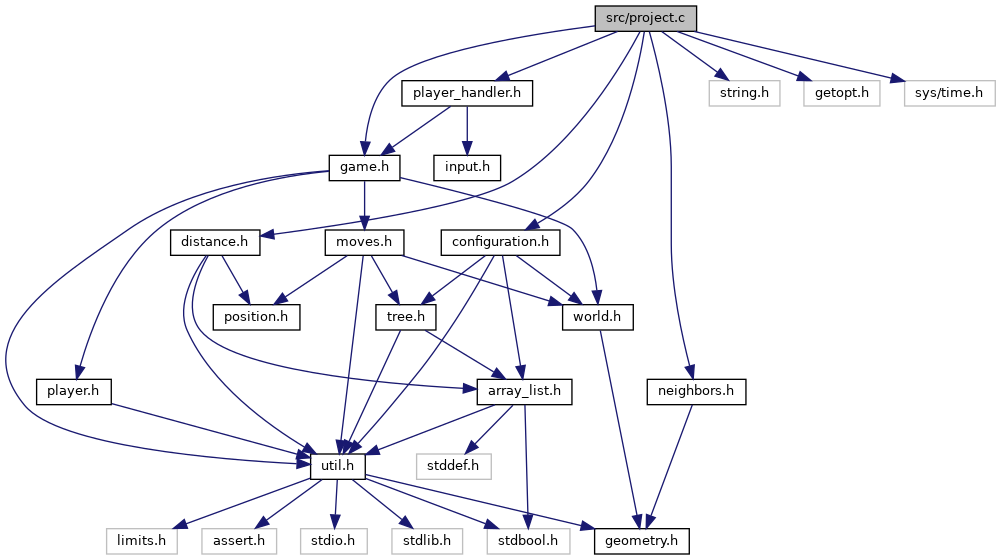
\includegraphics[width=\linewidth]{images/project_8c__incl.png}
\end{figure}



mettre graph dep


